\documentclass{article}
%
% Demo of the mcode package from 
% http://www.mathworks.co.uk/matlabcentral/fileexchange/8015-m-code-latex-package
% Updated 06 Mar 2014
%

\usepackage{graphicx}
\usepackage{wrapfig}
\usepackage{mathtools}
\usepackage{mathrsfs}
\usepackage{enumitem}
\usepackage{pdflscape}
\usepackage{color}
\usepackage{float}
\usepackage{amssymb}

\graphicspath{ {images/} }

% load package with ``framed'' and ``numbered'' option.
\usepackage[framed,numbered,autolinebreaks,useliterate]{mcode}

% something NOT relevant to the usage of the package.
\usepackage{url}
\setlength{\parindent}{0pt}
\setlength{\parskip}{18pt}


% //////////////////////////////////////////////////

\begin{document}

\title{Homework 6 - Optimal Control Systems}
\author{Erivelton Gualter dos Santos, 2703806}
\date{}

\maketitle 

\section{Find the point in 3D space}

Use the Lagrange multiplier technique to find the point in 3D space that is nearest the origin and that satisfies the constraints $x_1+x_2+x_3=5$, and $x_1^2+x_2^2+x_3=9$.

Using the \textit{Lagrange Multiplier Metho}d, we have the following \textit{augmented function}:
\begin{eqnarray*}
f_a(x_1,x_2,x_3,p_1,p_2)  \triangleq x_1^2+x_2^2+x_3^2 + p_1(x_1+x_2+x_3-5) + p_2(x_1^2+x_2^2+x_3-9)
\end{eqnarray*}
The necessary condition is: 
$$ df_a(x_1,x_2,x_3,p_1,p_2) = 0$$
Therefore:
\begin{eqnarray*}
\begin{split}
df_a(x_1,x_2,x_3,p_1,p_2) &= (2x_1+p1+2x_1p_2)\Delta x_1 + (2x_2+p1+2x_2p_2)\Delta x_2 + \\
& (2x_3+p1+p_2)\Delta x_3 + (x_1+x_2+x_3-5)\Delta p_1 + \\
& (x_1^2+x_2^2+x_3-9)\Delta p_2
\end{split}
\end{eqnarray*}

Therefore, it results in the following equations:
\begin{eqnarray}
\begin{split}
(2+2p_2)x_1 + p1 &= 0 \\
(2+2p_2)x_2 + p1 &= 0 \\
2x_3+p1+p_2 &= 0 \\
x_1+x_2+x_3 &= 5 \\
x_1^2+x_2^2+x_3 &= 9
\end{split}
\end{eqnarray}

From equations 1.1 and 1.2, we know that $x_1 = x_2$.

Subtracting equation 1.4 aper 1.3, we have $x_1^2-2x_1-2=0$. Therefore, $x_1$ has two solutions: $-1$ and $2$.

For $x_1 = -1$, we have $x_2 = -1$ and $x_3 = 7$. For $x_1 = 2$, we have $x_2 = 2$ and $x_3 = 1$. The nearest point to the origin is \textbf{(2,2,1)} and distance equal a 9.

\section{Find extremal}

\begin{equation*}
J(x) = \int_{0}^{1} \left[  \frac{1}{2}\dot{x}^2(t) + x(t)\dot{x}(t) + \dot{x}(t) + x(t) \right] dt
\end{equation*}

For $ x(0)=\frac{1}{1}$ and $x(1) = \:$free

The solution of this problem can be found using the Euler Equation:
\begin{eqnarray}
\frac{\partial g}{\partial y} - \frac{d}{dt}\frac{\partial q}{\partial \dot{y}} = 0
\end{eqnarray}
Therefore, for $g(x,\dot{x}, t) = \frac{1}{2}\dot{x}^2(t) + x(t)\dot{x}(t) + \dot{x}(t) + x(t)$, we have:
\begin{eqnarray*}
\begin{split}
\frac{\partial g}{\partial y} &= \dot{x}(t)+1 \\
\frac{\partial q}{\partial \dot{y}} &= \dot{x}(t)+ x(t)+1  \\
\frac{d}{dt}\frac{\partial q}{\partial \dot{y}} &= \ddot{x}(t) + \dot{x}(t) \\
\end{split}
\end{eqnarray*}
So, 
\begin{eqnarray*}
\ddot{x}(t) = 1
\end{eqnarray*}
The solution for this equation can be written as: $ x(t) = \frac{t^2}{2} + tC_1 + C_2$. Using the boundary condition:  $x(0)=\frac{1}{2}$, we have the following constant values: $C_1 = \frac{-3}{2}$ and $C_2 = \frac{1}{2}$.
So,
\begin{eqnarray}
x(t) = \frac{t^2}{2}-\frac{3}{2}t+\frac{1}{2}
\end{eqnarray}

\section{Catenary Problem}

Knowing that the equation of the hanging rope is: 
\begin{eqnarray}
y = h * (cosh(x / h) - cosh(a / 2 / h)) 
\end{eqnarray}
and the length constraint equation is: 
\begin{eqnarray}
L = 2 * h * sinh(a / 2/ h)
\end{eqnarray}

For $L=2.05$ , we can find \textit{h} from equation 3. Therefore, $h=2.5916$.

For $L=2.90$ , we can find \textit{h} from equation 3. Therefore, $h=0.6460$.

\begin{figure}[H]
\centering
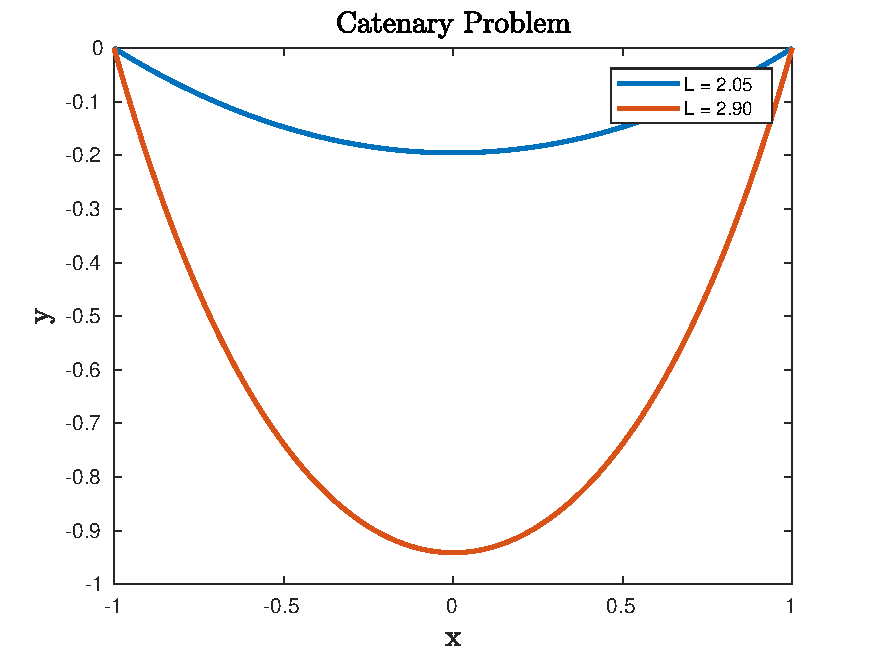
\includegraphics [width=4.4in]{f1}
\caption{Catenary Problem for L=2.05 and L=2.9}
\end{figure}

To find the "natural catenary", we need to find the shape and length of a hanging rope that minimizes potential energy without the a length constraint. 

Therefore, for a potential energy equal to: $PE = G\sigma\int_{-a/2}^{a/2} y\left( 1+\dot{y}^2 \right)^{1/2}dx$. 

So, as the $g(x,\dot{x})$ is not an explicit function of time, then $\dot{y}\frac{\partial g}{\partial \dot{y}} -g=K$.
So, for:
\begin{eqnarray*}
\frac{\partial g}{\partial \dot{y}} = y\dot{y}(1+\dot{y}^2)^{1/2}
\end{eqnarray*}
we have:
\begin{eqnarray*}
G\sigma y\dot{y}^2(1+\dot{y}^2)^{1/2}-G\sigma y\left( 1+\dot{y}^2 \right)^{1/2} = K
\end{eqnarray*}
Therefore, it results in:
\begin{eqnarray*}
\dot{y}^2 = \left(\frac{G\sigma y}{K}\right)^2 - 1
\end{eqnarray*}
The solution for this equation is the same as the one described in lecture notes; however, the value of $p$ and $p'$ is zero, so it results in:
\begin{eqnarray}
y = -h\cosh(\frac{x}{h})
\end{eqnarray}

Next, step is to find h parameter for the boundaries conditional. 

For the asked boundary condition, we have $y(-1)=y(+1)=0$. However, for this boundaries condition it is not possible to find the natural cantenary. Aiming tho observe the shape of the natural cantenary, it was solved for different boundaries condition and also it was shifted to the same y axis to observe if it has the same shape. In the following figure, you can check that the boundaries condition used was: $y(-1)=y(+1)=2,2.5,3,3.5,4,4.5$. You can observe that the length of the rope and the shape is also different. I assume as the boundary condition approaches positive infinity, the natural cantenary reaches a straight line and a length equal 2. In contrast, the graph becomes more concave and a slightly bigger L when the y approaches to zero.

\begin{figure}[H]
\centering
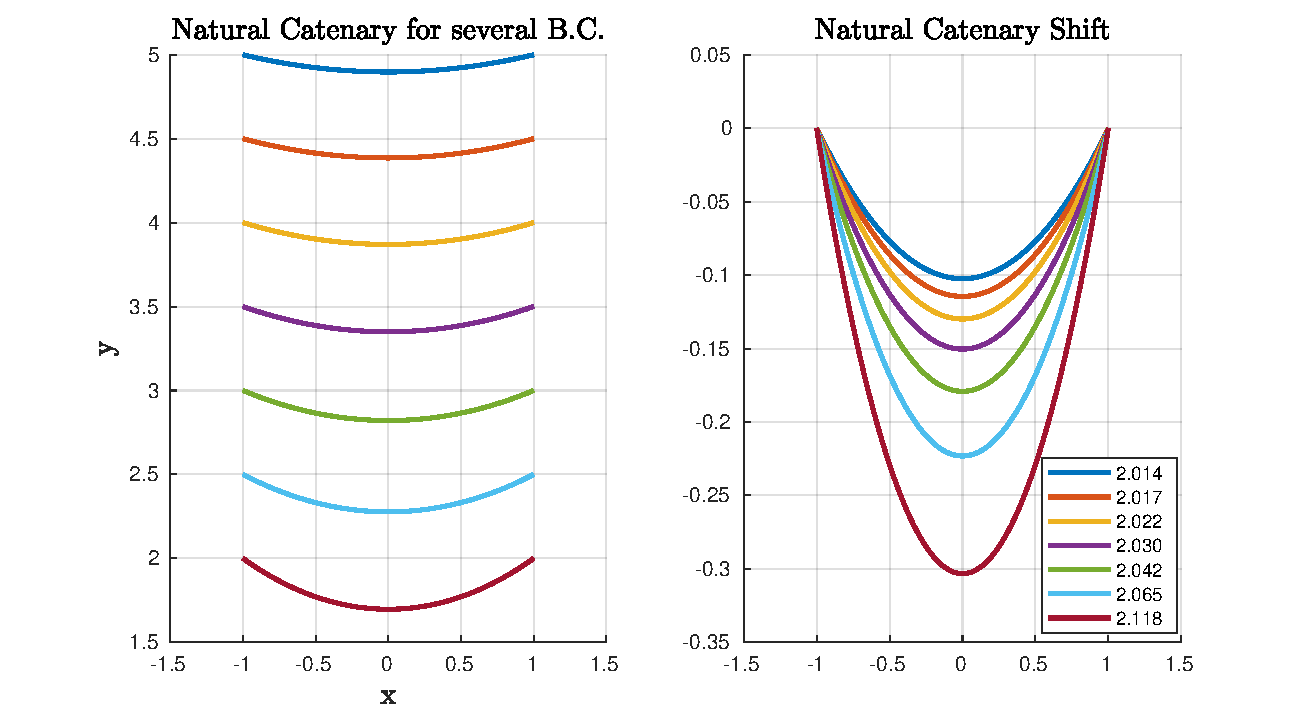
\includegraphics [width=4.in]{f4}
\caption{Catenary Problem for L=2.05 and L=2.9}
\end{figure}


\textbf{For the ground level is at y=-2, the length L for which the hanging rope will just barely touch the ground?}

The length for the hanging rope at a distance of 2 from the ground level is: 4.742.

\begin{figure}[H]
\centering
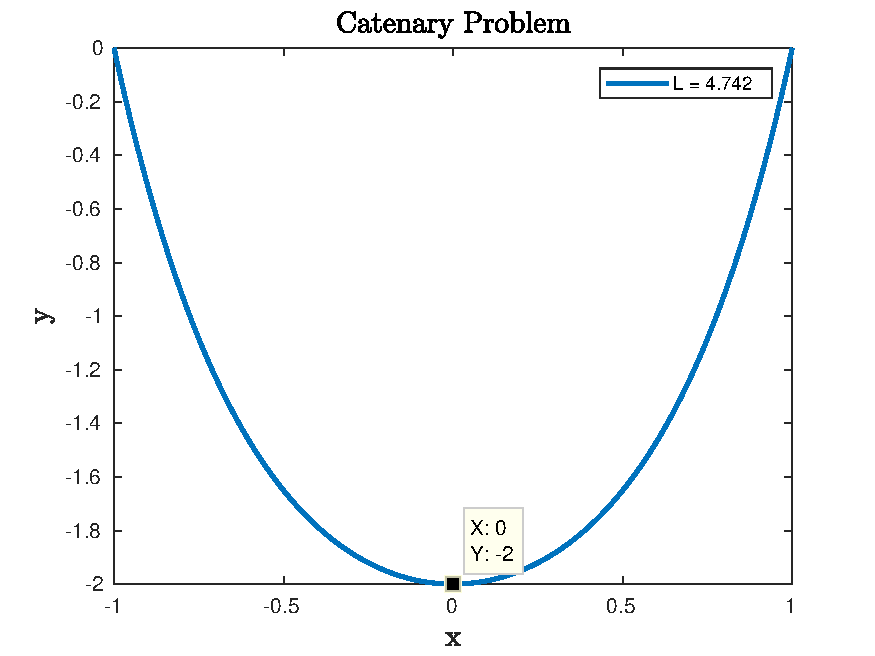
\includegraphics [width=4.4in]{f2}
\caption{Catenary Problem}
\end{figure}


\section{Dido's problem}

The dido's problem is a isoperimetric optimization problem which means it is the optimisation of a function under the constraint of an integral. As the problem aiming to maximize the cost function which is the area under the curve, this shape (or function) should have a single value of x for the value of y. When $L$ is bigger than $p*\pi$, the center of the circle is above the x axis, so for a set of x it has two points in the image axis. Therefore, if we solve the area under the curve between the x limits, the area outside this limits will be not counted as the following image. For this reason, the circle equation is just valid for $L < p*\pi$.

\begin{figure}[H]
\centering
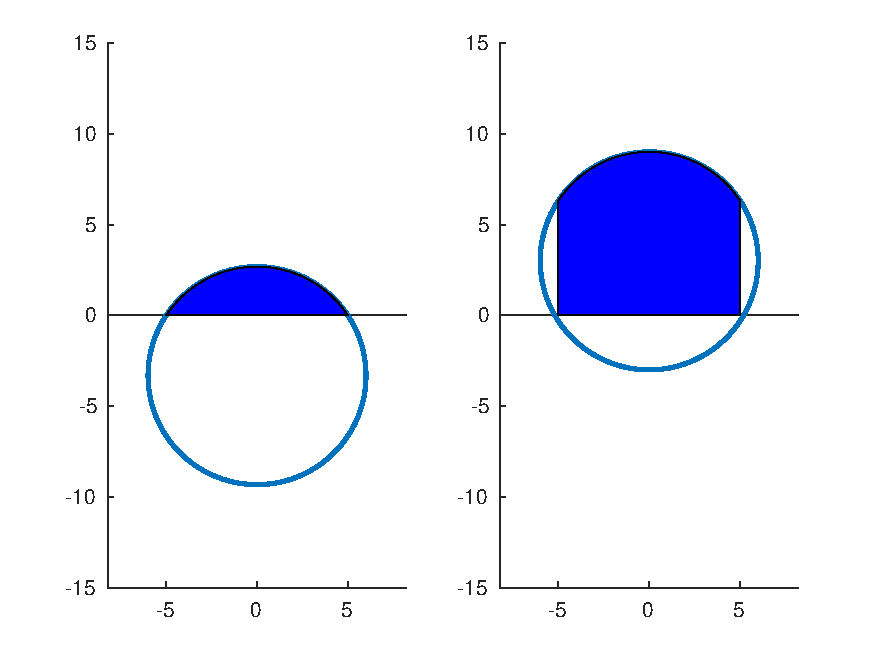
\includegraphics [width=4.4in]{f3}
\caption{Dido's Problem}
\end{figure}


\begin{lstlisting}
% Book: Optimal Control Theory: An introduxtion by Donald E. Kirk
%
% Erivelton Gualter, 02/28/2018

clear all; clc; close all

%% Question 3-a
a = 2;

myfun = @(L,h,a) L - 2 * h * sinh(a / 2/ h);
 
L = 2.05; fun1 = @(h) myfun(L,h,a); h1 = fzero(fun1,0.1); h1=abs(h1);
L = 2.90; fun2 = @(h) myfun(L,h,a); h2 = fzero(fun2,0.1); h2=abs(h2);

x = -a/2:0.01:a/2; 

y1 = h1 * (cosh(x / h1) - cosh(a / 2 / h1));
y2 = h2 * (cosh(x / h2) - cosh(a / 2 / h2));

f1 = figure; plot(x, y1, x, y2, 'LineWidth', 2); 

title('Catenary Problem', 'Interpreter','Latex', 'FontSize',14);
xlabel('x', 'Interpreter','Latex', 'FontSize',14);
ylabel('y', 'Interpreter','Latex', 'FontSize',14);
legend('L = 2.05', 'L = 2.90');

%% Question 3 - natural catenary
f4 = figure; hold on
ax1 = subplot(121); 
ax2 = subplot(122);
%% 
a = 2; syms h;
dy = 2; % 2, 2.5, 3, 3.5, 4, 4.5, 5
hn = vpasolve(h * cosh(a / 2 / h) == dy, h ); 
Ln =  2 * hn * sinh(a / 2 / hn)
yn = hn * (cosh(x / hn));
yn2 = hn * (cosh(x / hn))-dy;

hold(ax1,'on'); plot(ax1, x, yn, 'LineWidth', 2);  hold(ax1,'off')
    title(ax1, 'Natural Catenary for several B.C.', 'Interpreter','Latex', 'FontSize',14);
    xlabel(ax1, 'x', 'Interpreter','Latex', 'FontSize',14);
    ylabel(ax1, 'y', 'Interpreter','Latex', 'FontSize',14);
    xlim(ax1,[-1.5 1.5]);
    grid(ax1,'on')
    
hold(ax2,'on'); plot(ax2, x, yn2, 'LineWidth', 2);  hold(ax2,'off')
    title(ax2,'Natural Catenary Shift', 'Interpreter','Latex', 'FontSize',14);
    xlabel(ax1, 'x', 'Interpreter','Latex', 'FontSize',14);
    ylabel(ax1, 'y', 'Interpreter','Latex', 'FontSize',14);
    xlim(ax2,[-1.5 1.5]);
    grid(ax2,'on')

saveFigureToPdf('f4',f4);

%% Question 3-b
syms h
h3 = vpasolve(-h * (cosh(0 / h) - cosh(a / 2 / h)) == 2, h );

L3 = 2 * h3 * sinh(a / 2/ h3);

y3 = h3 * (cosh(x / h3) - cosh(a / 2 / h3));

f2 = figure; plot(x, y3, 'LineWidth', 2); 

title('Catenary Problem', 'Interpreter','Latex', 'FontSize',14);
xlabel('x', 'Interpreter','Latex', 'FontSize',14);
ylabel('y', 'Interpreter','Latex', 'FontSize',14);
legend(['L = ' num2str(double(L3))]);

saveFigureToPdf('f2',f2);

%% Question 4
close all
r = 6; a = 5; 

f3 = figure;
subplot(121);
y = -4+0.6823;
circle(0,y,r); 
semicrc = r.*[cos(acos(a/r):0.01:(pi-acos(a/r))); ...
              sin(acos(a/r):0.01:(pi-acos(a/r)))];
semicrc(2,:) = semicrc(2,:) + y;

area(semicrc(1,:), semicrc(2,:), 'FaceColor','b')
axis([-6 6 -15 15]); axis equal

subplot(122);
y = 3;
circle(0,y,r); 
semicrc = r.*[cos(acos(a/r):0.01:(pi-acos(a/r))); ...
              sin(acos(a/r):0.01:(pi-acos(a/r)))];
semicrc(2,:) = semicrc(2,:) + y;

area(semicrc(1,:), semicrc(2,:), 'FaceColor','b')
axis([-6 6 -15 15]); axis equal
saveFigureToPdf('f3',f3);

\end{lstlisting}

You can access the code at: https://github.com/EriveltonGualter/EEC-744-Optimal-Control-Systems

\end{document}
